% XCircuit output "block.tex" for LaTeX input from block.ps
\def\putbox#1#2#3#4{\makebox[0in][l]{\makebox[#1][l]{}\raisebox{\baselineskip}[0in][0in]{\raisebox{#2}[0in][0in]{\scalebox{#3}{#4}}}}}
\def\rightbox#1{\makebox[0in][r]{#1}}
\def\centbox#1{\makebox[0in]{#1}}
\def\topbox#1{\raisebox{-0.60\baselineskip}[0in][0in]{#1}}
\def\midbox#1{\raisebox{-0.20\baselineskip}[0in][0in]{#1}}
   \scalebox{1}{
   \normalsize
   \parbox{8.16667in}{
   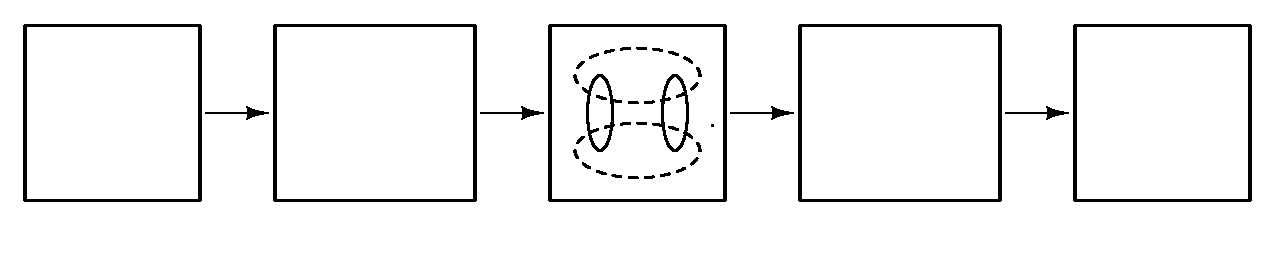
\includegraphics[scale=1]{block.eps}\\
   % translate x=544 y=432 scale 0.38
   \tiny
   \putbox{1.81in}{0.97in}{1.20}{RF Power}%
   \putbox{5.31in}{0.97in}{1.20}{RF to DC}%
   \putbox{5.31in}{0.64in}{1.20}{Converter}%
   \putbox{7.31in}{0.81in}{1.20}{Load}%
   \putbox{1.81in}{0.64in}{1.20}{Generator}%
   \putbox{0.31in}{0.64in}{1.20}{Power}%
   \putbox{0.31in}{0.97in}{1.20}{Mains}%
   \putbox{3.89in}{0.06in}{1.20}{Coils}%
   } % close 'parbox'
   } % close 'scalebox'
   \vspace{-\baselineskip} % this is not necessary, but looks better
